% 1977 年广西百色卷（理科）第五题：三角形 ABC 的三边 a、b、c，
% AD 为 BC 边上的高（虚线）（按源卷第 4 页布局）
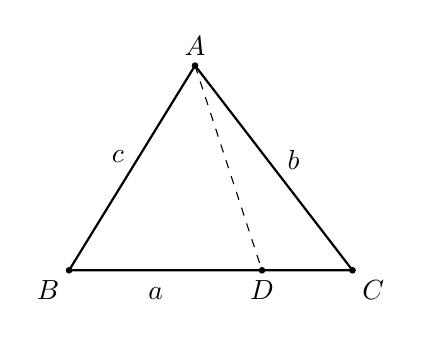
\begin{tikzpicture}[scale=1.0]
  \coordinate (A) at (1.6,2.6);
  \coordinate (B) at (0,0);
  \coordinate (C) at (3.6,0);
  \coordinate (D) at (2.45,0); % 高的垂足
  \draw[thick] (A)--(B)--(C)--cycle;
  \draw[dashed] (A)--(D);
  \fill (A) circle (1.2pt) node[above] {$A$};
  \fill (B) circle (1.2pt) node[below left] {$B$};
  \fill (C) circle (1.2pt) node[below right] {$C$};
  \fill (D) circle (1.2pt) node[below] {$D$};
  \node at (0.62,1.45) {$c$};
  \node at (2.85,1.40) {$b$};
  \node at (1.10,-0.30) {$a$};
\end{tikzpicture}
